\section{$\Vzero$ Efficiency Calculation with the Weighting Approach}
\label{sec:a01WghtV0Effi}

There is an alternative weighting approach for the JC and OC $\Vzero$
efficiency calculation in addition to the scaling approach,
which introduced in section~\ref{sec:c05ScaledV0Effi},
is also studied in this analysis.

The strategy of this approach is:
\begin{enumerate}
\item build the $\pT-\eta$ 2D weight according to the ratio of the
      differential distribution of JC (or OC) $\Vzero$ and that of
      inclusive $\Vzeros$,
      \begin{equation}
      w_{\rm JC/OC}=\frac{{\rm d}^{2}N_{\rm JC/OC}/{\rm d}\pT{\rm d}\eta}
                         {{\rm d}^{2}N_{\rm inclu}/{\rm d}\pT{\rm d}\eta}
      \end{equation}
      as an example shown in figure~\ref{fig:a01V0ProbWgt};
\item use $w_{\rm JC/OC}$ as a weight in the calculation of the $\Vzero$
      efficiency,
      \begin{equation}
      \varepsilon_{\rm JC/OC}=
      \frac{\sum_{\eta}w_{\rm JC/OC}(\pT,\eta)\times N_{\Vzero}^{\rm reco}}
           {\sum_{\eta}w_{\rm JC/OC}(\pT,\eta)\times N_{\Vzero}^{\rm kine}}.
\end{equation}
\end{enumerate}

\begin{figure}[htb]
\begin{center}
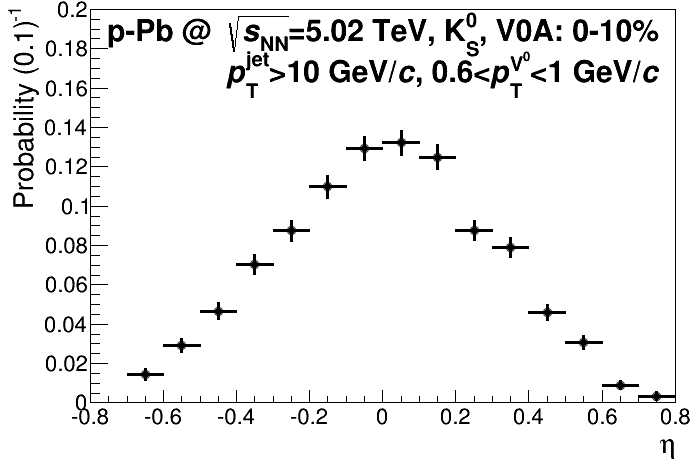
\includegraphics[width=.48\textwidth]{a01EffiV0Wgt/cProbability}
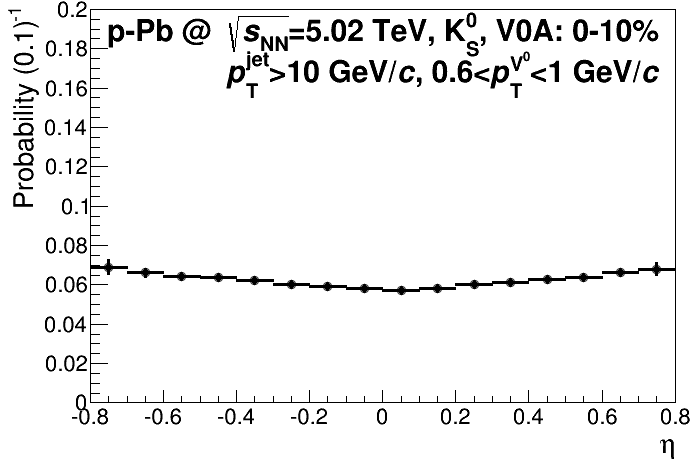
\includegraphics[width=.48\textwidth]{a01EffiV0Wgt/cProbability_OC}
\caption{The $w_{\rm JC/OC}(\pT,\eta)$ distriubtion of $\Kshort$
         defined in eq.~(\ref{eq:a01V0Wgt}) in $0.6<\pT<1~\GeVc$.}
\label{fig:a01V0ProbWgt}
\end{center}
\end{figure}

\begin{figure}[htb]
\begin{center}
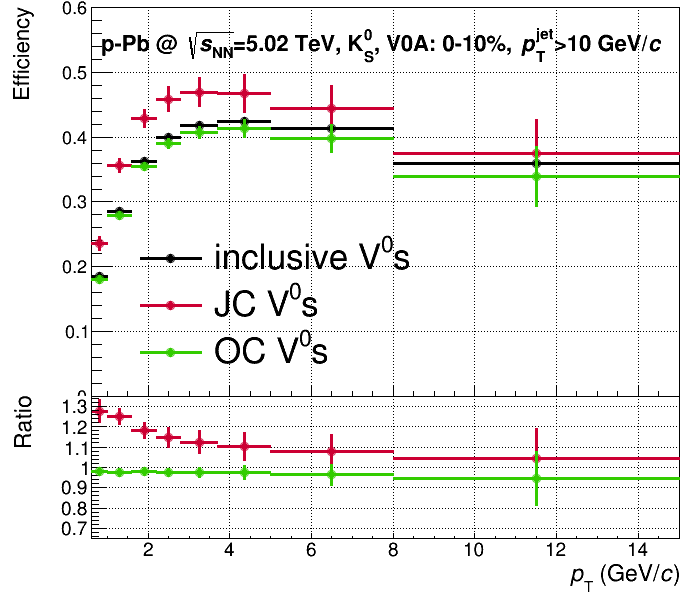
\includegraphics[width=.32\textwidth]{a01EffiV0Wgt/cKshortV0A000010PtJ10}
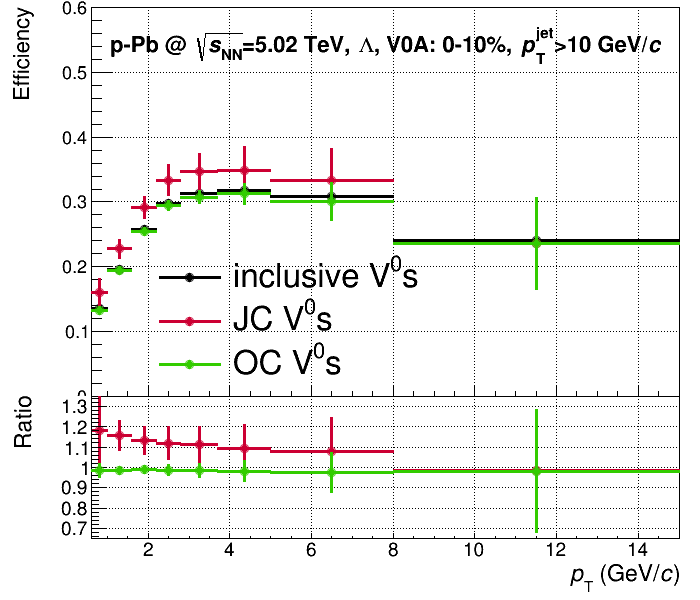
\includegraphics[width=.32\textwidth]{a01EffiV0Wgt/cLambdaV0A000010PtJ10}
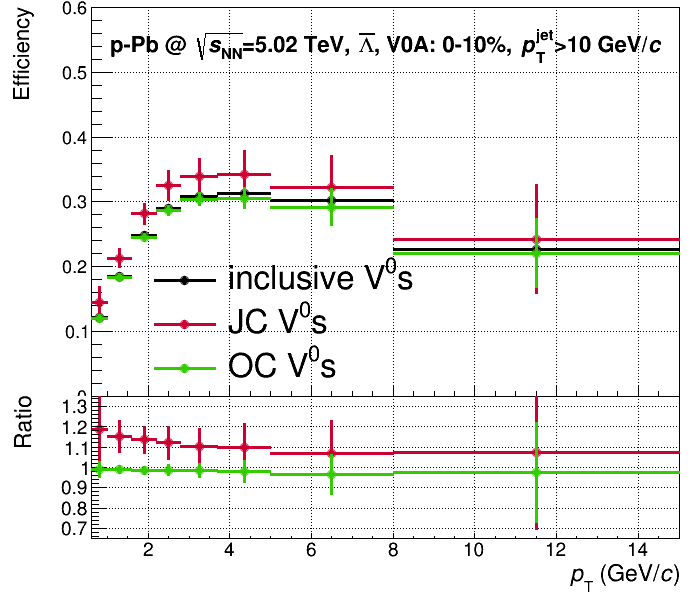
\includegraphics[width=.32\textwidth]{a01EffiV0Wgt/cAntiLaV0A000010PtJ10}
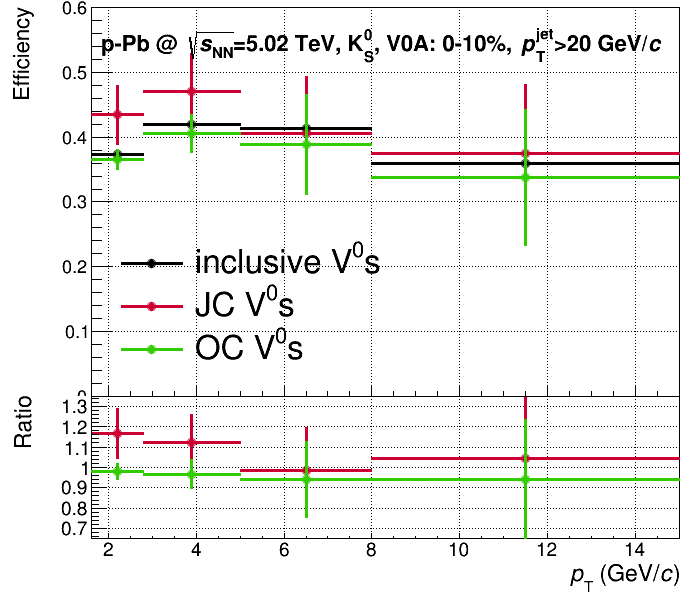
\includegraphics[width=.32\textwidth]{a01EffiV0Wgt/cKshortV0A000010PtJ20}
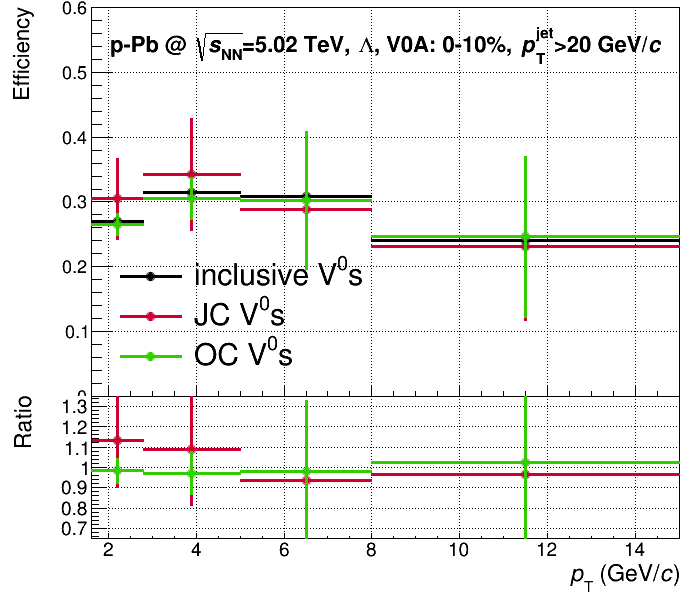
\includegraphics[width=.32\textwidth]{a01EffiV0Wgt/cLambdaV0A000010PtJ20}
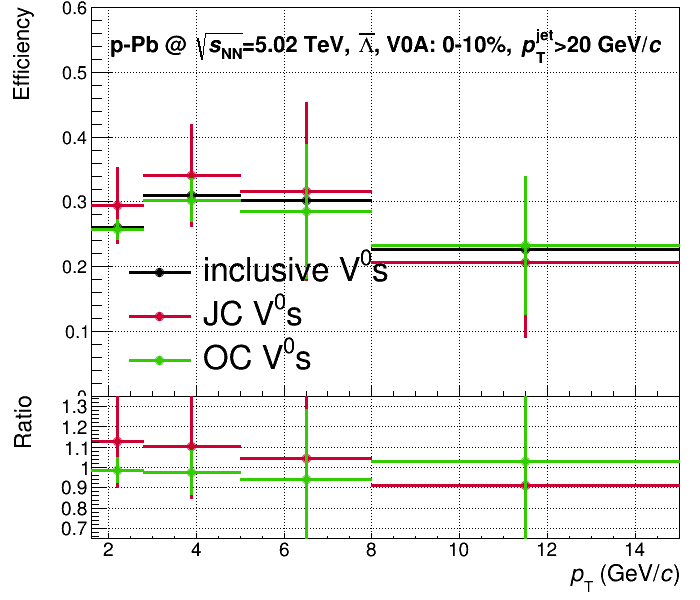
\includegraphics[width=.32\textwidth]{a01EffiV0Wgt/cAntiLaV0A000010PtJ20}
\caption{Efficiency of JC and OC $\Vzeros$ in $\pT^{\rm jet}>10~\GeVc$ (upper)
         and $\pT^{\rm jet}>20~\GeVc$ (lower) in $0-10\%$.
         Results are compared to the inclusive $\Vzeros$.}
\label{fig:a01EffiJEV0s000010}
\end{center}
\end{figure}

\begin{figure}[htb]
\begin{center}
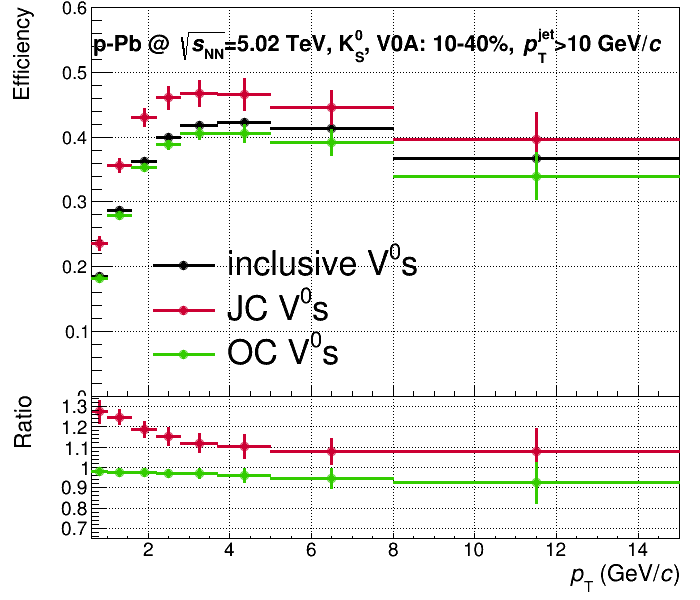
\includegraphics[width=.32\textwidth]{a01EffiV0Wgt/cKshortV0A010040PtJ10}
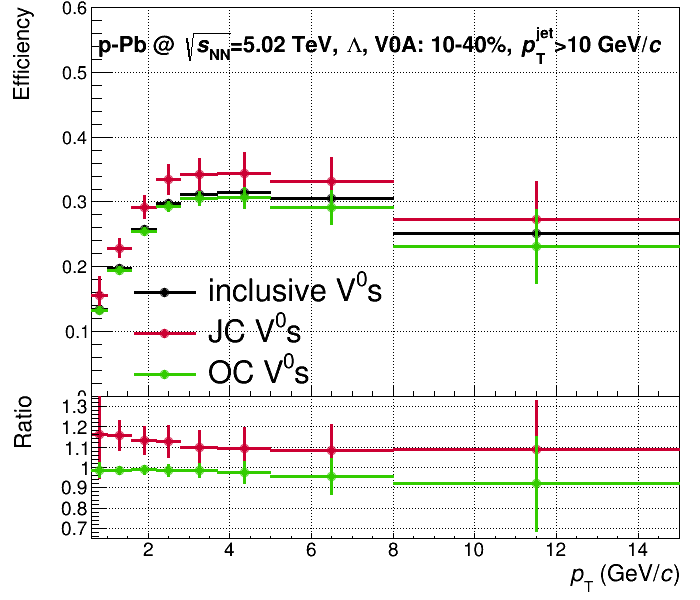
\includegraphics[width=.32\textwidth]{a01EffiV0Wgt/cLambdaV0A010040PtJ10}
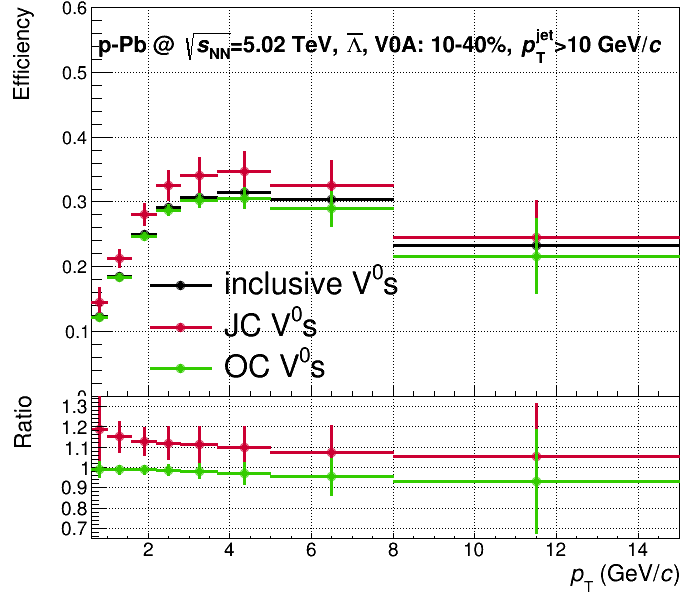
\includegraphics[width=.32\textwidth]{a01EffiV0Wgt/cAntiLaV0A010040PtJ10}
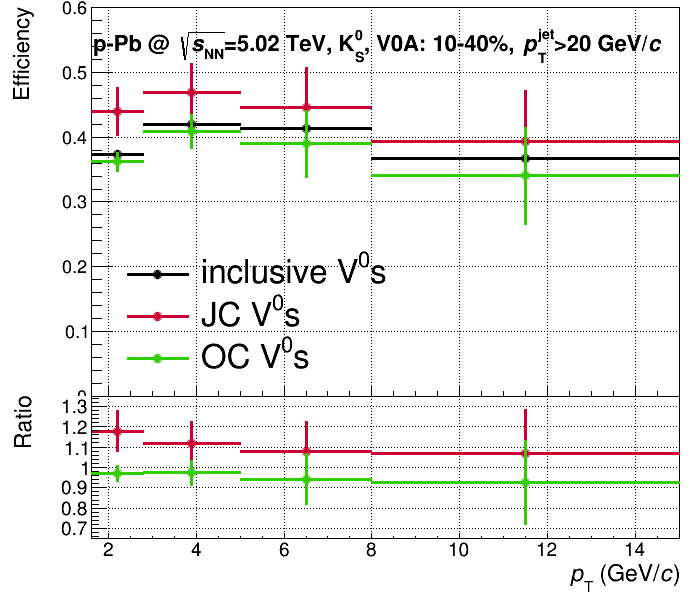
\includegraphics[width=.32\textwidth]{a01EffiV0Wgt/cKshortV0A010040PtJ20}
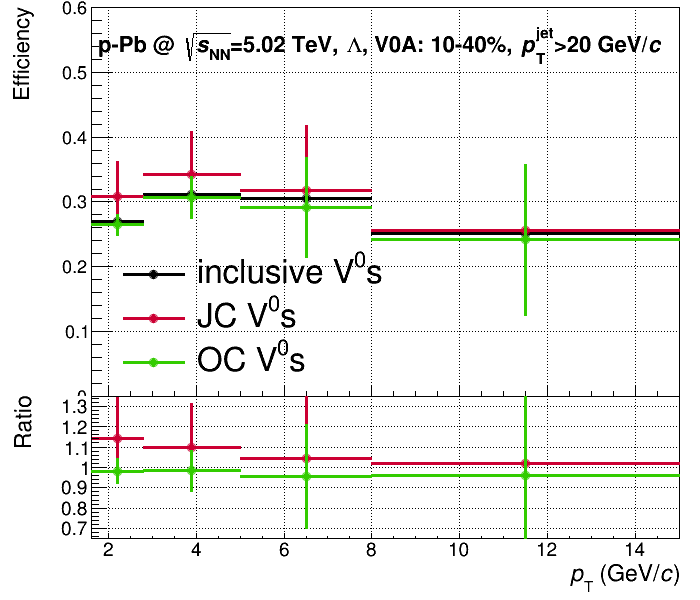
\includegraphics[width=.32\textwidth]{a01EffiV0Wgt/cLambdaV0A010040PtJ20}
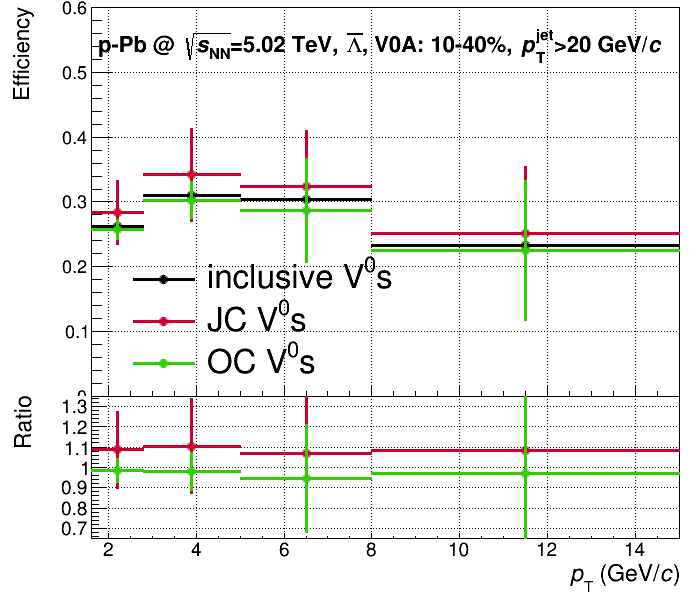
\includegraphics[width=.32\textwidth]{a01EffiV0Wgt/cAntiLaV0A010040PtJ20}
\caption{Efficiency of JC and OC $\Vzeros$ in $\pT^{\rm jet}>10~\GeVc$ (upper)
         and $\pT^{\rm jet}>20~\GeVc$ (lower) in $10-40\%$.
         Results are compared to the inclusive $\Vzeros$.}
\label{fig:a01EffiJEV0s010040}
\end{center}
\end{figure}

\begin{figure}[htb]
\begin{center}
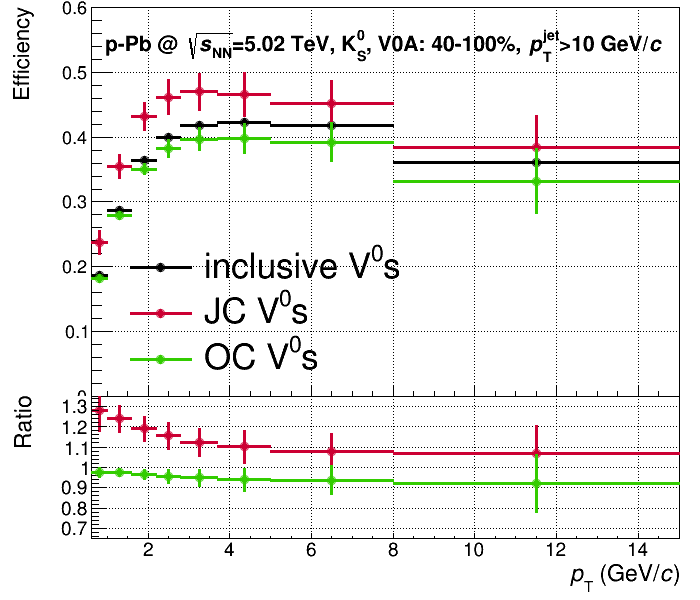
\includegraphics[width=.32\textwidth]{a01EffiV0Wgt/cKshortV0A040100PtJ10}
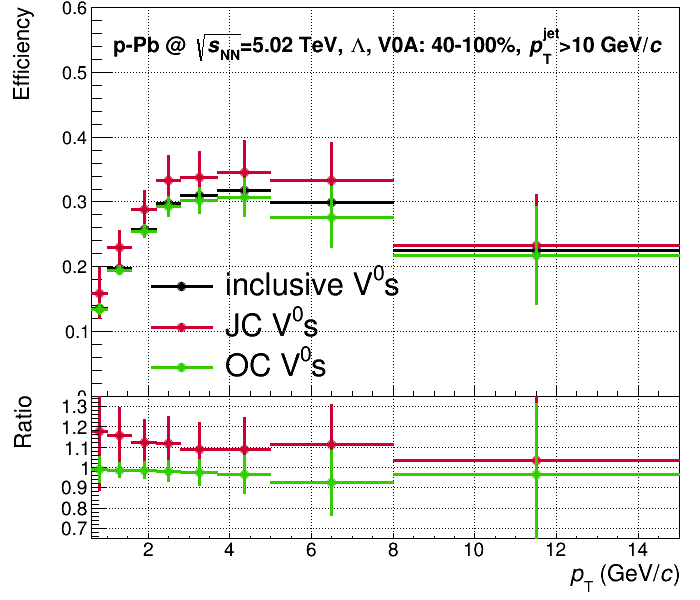
\includegraphics[width=.32\textwidth]{a01EffiV0Wgt/cLambdaV0A040100PtJ10}
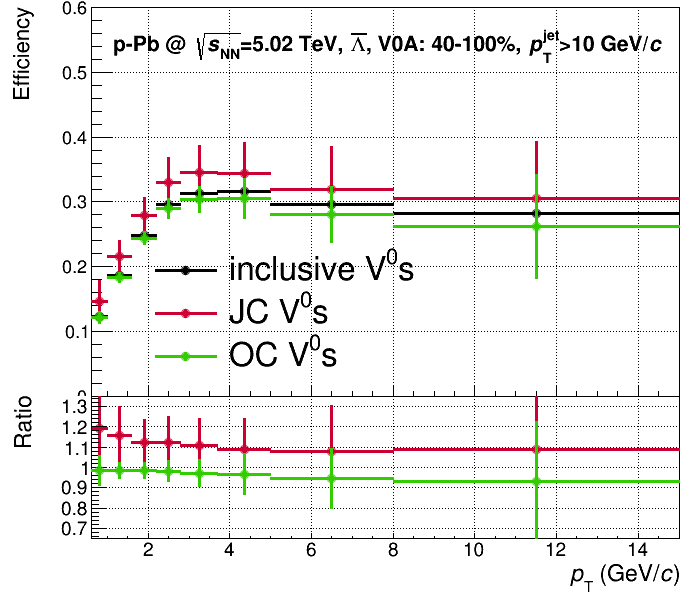
\includegraphics[width=.32\textwidth]{a01EffiV0Wgt/cAntiLaV0A040100PtJ10}
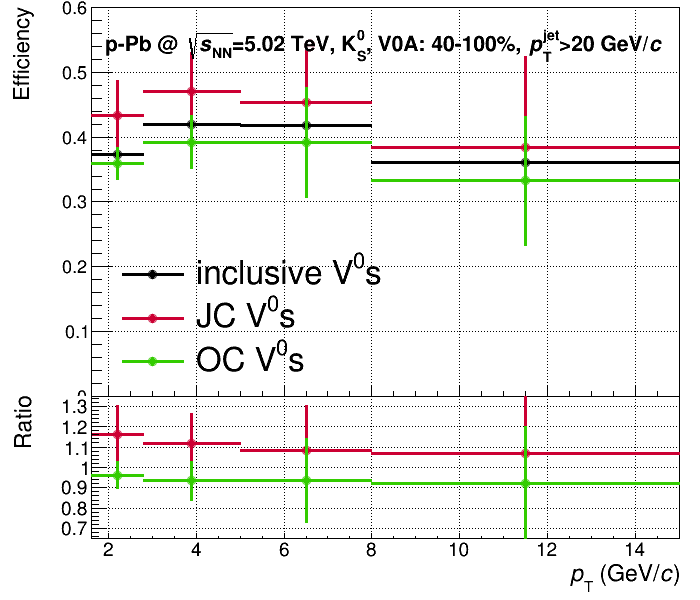
\includegraphics[width=.32\textwidth]{a01EffiV0Wgt/cKshortV0A040100PtJ20}
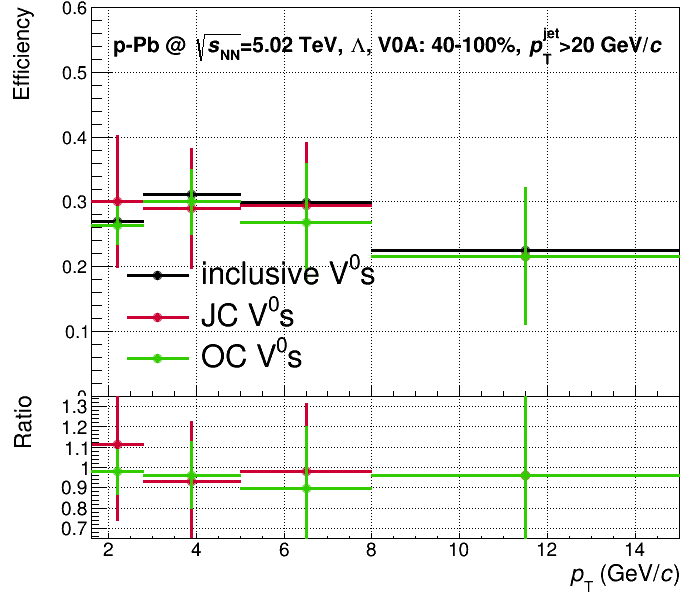
\includegraphics[width=.32\textwidth]{a01EffiV0Wgt/cLambdaV0A040100PtJ20}
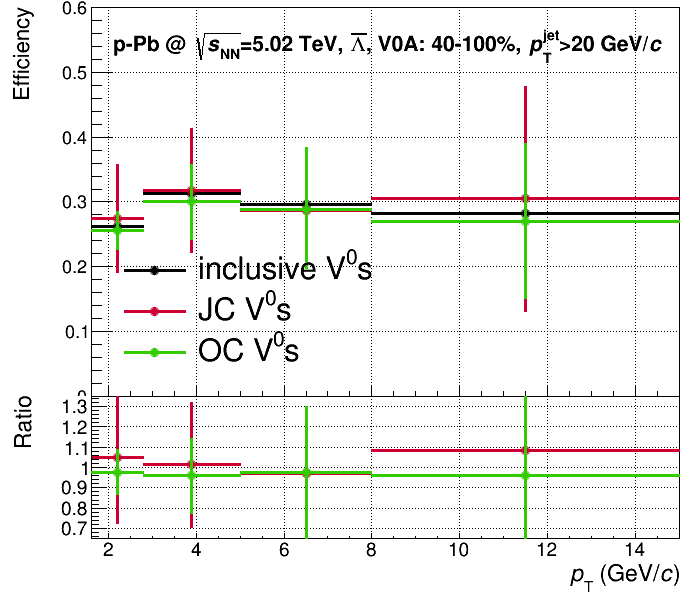
\includegraphics[width=.32\textwidth]{a01EffiV0Wgt/cAntiLaV0A040100PtJ20}
\caption{Efficiency of JC and OC $\Vzeros$ in $\pT^{\rm jet}>10~\GeVc$ (upper)
         and $\pT^{\rm jet}>20~\GeVc$ (lower) in $40-100\%$.
         Results are compared to the inclusive $\Vzeros$.}
\label{fig:a01EffiJEV0s040100}
\end{center}
\end{figure}

The efficiency of JC and OC (with $\Delta R>0.6$) $\Vzeros$
in $\pT^{\rm jet}>10~\GeVc$ and $\pT^{\rm jet}>20~\GeVc$
in three event multiplicity bins
are shown in figure~\ref{fig:a01EffiJEV0s000010}
to figure~\ref{fig:a01EffiJEV0s040100}.
The r esults are compared to the inclusive $\Vzeros$.
The efficiency of $\Kshort$ ($\Lambda$) in jets is
$\sim 10-30\%$ ($\sim 10-20\%$) larger than that of the inclusive $\Vzeros$.
The efficiency of OC $\Vzeros$ is almost the same as that of
the inclusive $\Vzeros$.
